\documentclass[a4paper]{article}
\usepackage{graphicx}  % Allows inclusion of images
\usepackage{geometry}  % Manages page layout
\usepackage{calc}      % Enables calculations in LaTeX
\usepackage{multicol}  % Supports multiple column layout
\usepackage{enumitem}  % Customizes list environments
\usepackage{xcolor}    % Enables color manipulation
\usepackage{fontspec}  % Supports custom fonts
\usepackage{tcolorbox} % Creates colored boxes
\usepackage[svgnames]{xcolor} % Provides named colors
\usepackage{lipsum}  

% Load custom font from the 'font' directory
\newfontface\fontseasons[Path=./fonts/]{TheSeasonsRegular.otf}

% Set PublicSans as the main font with variations
\setmainfont[
Path=./fonts/,                  % Path to font files
UprightFont = *-Regular.ttf,    % Regular font
BoldFont    = *-Bold.ttf,       % Bold weight
ItalicFont  = *-Italic.ttf,     % Italic style
BoldItalicFont = *-BoldItalic.ttf % Bold + Italic
]{PublicSans}

% Recipe details
\newcommand{\recipeName}{Soboro Don}
\newcommand{\servings}{4}
\newcommand{\prepTime}{120 MIN}
\newcommand{\cookTime}{20 MIN}
\newcommand{\recipeImage}{./images/soboro}


% Define layout measurements
\newlength{\picmargin}
\setlength{\picmargin}{15pt}
\newlength{\picwidth}
\setlength{\picwidth}{\paperwidth - 2\picmargin}

% Configure page geometry
\geometry{
	top=0pt,
	bottom=\picmargin,
	left=\picmargin,
	right=\picmargin,
	textwidth=\picwidth
}

% Define color scheme
\definecolor{bgIngredients}{HTML}{F8ECE9} 
\definecolor{Pagebackground}{HTML}{eeeeee}
\definecolor{captionColor}{HTML}{000000}
\definecolor{textColor}{HTML}{000000}
\definecolor{pinkTable}{HTML}{f8ece9}
\definecolor{shadecolor}{named}{pinkTable}
\pagecolor{Pagebackground} % Set background color

% Define command for recipe title styling
\newcommand{\recipeTitle}{
	\vspace{0.2cm}
	\parbox{\picwidth}{
		\centering
		\fontsize{28}{32}\selectfont\fontseasons{\recipeName}
	}
}

% Define command for ingredients
\newcommand{\ingredient}[1]{
	\item[]{#1}\\
}

\newcommand{\hide}[1]{} % Command to hide text

% Define environment for instructions section
\newenvironment{steps}
{
	{\fontsize{22}{26}\selectfont\fontseasons Instructions}
	\begin{enumerate}[leftmargin=0.4cm]
	}
	{
	\end{enumerate}
}

% Define ingredients box with layout adjustments

\newenvironment{ingredients}
{
	\vspace{-32.8pt} % Adjusts vertical positioning
	\begin{tcolorbox}[colback=bgIngredients, colframe=bgIngredients, width=\textwidth, boxsep=4pt, sharp corners, height=14cm, top=15pt]
		{\fontsize{22}{26}\selectfont\fontseasons Ingredients}
		\begin{itemize}[nosep, itemsep=-6pt, leftmargin=1pt]
			\vspace{5.4pt}
			\fontsize{10}{14}
		}
		{
		\end{itemize}
	\end{tcolorbox}
}


\begin{document}
	\pagestyle{empty} % Remove default headers and footers
	
	\begin{center}
		\makebox[\textwidth]{\includegraphics[width=\paperwidth]{\recipeImage}} % Add image
	\end{center}
	
	\color{textColor} % Set text color
	\vspace{0.6cm}
	\hspace{-\picmargin}
	\recipeTitle % Set recipe title
	
	\begin{center}
		\begin{tabular}{c c c}
			\fontsize{12}{16}\selectfont{SERVINGS: \servings}  \hspace{2.5cm} & \fontsize{12}{16}\selectfont{PREPPING TIME: \prepTime} & \hspace{.5cm} \fontsize{12}{16}\selectfont{COOKING TIME: \cookTime}
		\end{tabular}
		\vspace{2pt} % Adjust spacing
		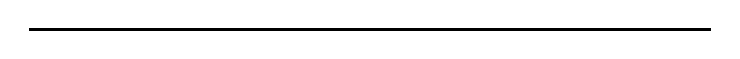
\begin{tikzpicture}
			\draw[very thick] (4,0) -- (\linewidth+15pt,0); % Draw horizontal line
		\end{tikzpicture}
	\end{center}
	\vspace{10pt} % Space between line and columns
	\setlength{\columnsep}{-100pt} % Adjust column separation
	\begin{multicols}{2} % Two-column layout
		\normalsize
		\raggedright
		\hspace{32pt}
		\begin{minipage}[t]{0.30\textwidth} % Allocate space for ingredients
			\begin{ingredients}
				\ingredient{250g thinly sliced beef strips}
				\ingredient{1.5 teaspoons unsweetened cocoa}
				\ingredient{1 cup butter (do not use margarine)}
				\ingredient{3 tablespoons vegetable oil}
				\ingredient{0.75 cups sugar}
				\ingredient{0.25 tablespoons pure vanilla extract}
			\end{ingredients}
		\end{minipage}
		
		\begin{minipage}[t]{0.49\textwidth} % Allocate space for instructions
			\begin{steps}
				\item{Lorem ipsum dolor sit amet, consetetur sadipscing elitr, sed diam nonumy eirmod tempor invidunt ut labore et dolore magna aliquyam erat, sed diam voluptua.}
				\item{At vero eos et accusam et justo duo dolores et ea rebum. Stet clita kasd gubergren, no sea takimata sanctus est Lorem ipsum dolor sit amet. Lorem ipsum dolor sit amet, consetetur sadipscing elitr, sed diam nonumy eirmod tempor invidunt ut labore et dolore magna aliquyam erat, sed diam voluptua.}
				\item{At vero eos et accusam et justo duo dolores et ea rebum. Stet clita kasd gubergren, no sea takimata sanctus est Lorem ipsum dolor sit amet. Lorem ipsum dolor sit amet, consetetur sadipscing elitr, sed diam nonumy eirmod tempor invidunt ut labore et dolore magna aliquyam erat, sed diam voluptua.}
				\item{At vero eos et accusam et justo duo dolores et ea rebum. Stet clita kasd gubergren, no sea takimata sanctus est Lorem ipsum dolor sit amet.}
				\item{Duis autem vel eum iriure dolor in hendrerit in vulputate velit esse molestie consequat, vel illum dolore eu feugiat nulla facilisis at vero eros et accumsan et iusto odio dignissim qui blandit praesent luptatum zzril delenit augue duis dolore te feugait nulla facilisi.}
				\item{Lorem ipsum dolor sit amet, consectetuer adipiscing elit, sed diam nonummy nibh euismod tincidunt ut laoreet dolore magna aliquam erat volutpat.}		
			\end{steps}
		\end{minipage}
	\end{multicols}
\end{document}
